\documentclass[tikz,border=3mm]{standalone}
\usepackage{newtxtext,newtxmath,pgfplots}
\pgfplotsset{compat=1.18}
\definecolor{NoteAccent}{HTML}{246A70}
\definecolor{NoteRule}{HTML}{D3DFE0}
\begin{document}
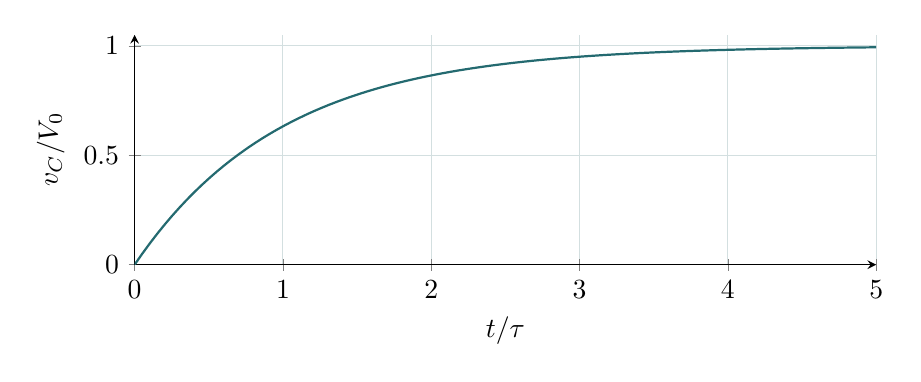
\begin{tikzpicture}
  \begin{axis}[width=11cm,height=4.5cm,axis lines=left,
    xmin=0,xmax=5,ymin=0,ymax=1.05,grid=major,
    grid style={NoteRule},xlabel={$t/\tau$},ylabel={$v_C/V_0$},
    xtick={0,1,2,3,4,5},ytick={0,0.5,1}]
    \addplot[NoteAccent,thick,domain=0:5,samples=100]
      {1-exp(-x)};
  \end{axis}
\end{tikzpicture}
\end{document}
